\subsection{Jet internal structure}\label{sec:jetsub}
The first measurements of jet quenching through full jet reconstruction at the LHC revolutionized our understanding of parton energy loss in a hot and dense medium. Nevertheless, there remains a gap in our understanding of the jet quenching mechanism that could be resolved by measuring the exact properties of the parton evolution through the medium. High statistics of collected jets during HL-LHC will provide a prime opportunity to explore the details of the internal structure of high energy jets that undergo interactions with the QGP. Observables probing the internal structure of jets can be defined using all measured hadrons in a jet or by using subjet techniques selecting only a specific region of the radiation phase space. In the following sections both approaches and their potential will be discussed.

\subsubsection{Substructure with hadrons}
Inclusive measurements of the longitudinal and transverse momentum distribution of hadrons in inclusive jets have been performed with high accuracy at the LHC~\cite{Aaboud:2018hpb,Sirunyan:2018jqr}. The modification due to jet quenching is studied by comparing the results in pp and Pb--Pb collisions.
%At the edges of the phase space
For certain kinematic selections, for example at large $z$ where the leading particle in the jet is carrying a large fraction of the total jet momentum, the current experimental uncertainties are however large (see left panel of Fig.~\ref{fig:jetDz}) limiting the constraints on the jet quenching mechanism that can be extracted by comparing data to theoretical models. The expected statistical precision at HL-LHC for the ratio of fragmentation functions in Pb--Pb and pp collisions is shown in Fig.~\ref{fig:jetDz}. This precision will allow to characterize in detail the excess in yield of hard (large $z$) and soft (small $z$) fragments and the suppression in the region between these two excesses providing strong constraints to theoretical models. Measurements of the rapidity dependence of jet observables are of great interest since the fraction of quark- and gluon-initiated jets varies with rapidity. However, current measurements of the fragmentation function are statistics limited and no significant rapidity dependence is observed~\cite{Aaboud:2018hpb}. The right panel of Fig.~\ref{fig:jetDz} shows the ratio of fragmentation functions of high momentum jets for most central collisions with the expected accuracy at the HL-LHC. The projection are compared to the hybrid model~\cite{Casalderrey-Solana:2014bpa,Hulcher:2017cpt} which implements energy loss according to the strong coupling description of the radiation of low energy gluons associated with the hot QCD matter which predicts a rapidity-dependent suppression of particle yield at high $z$. 
\begin{figure}[!ht]
\begin{center}
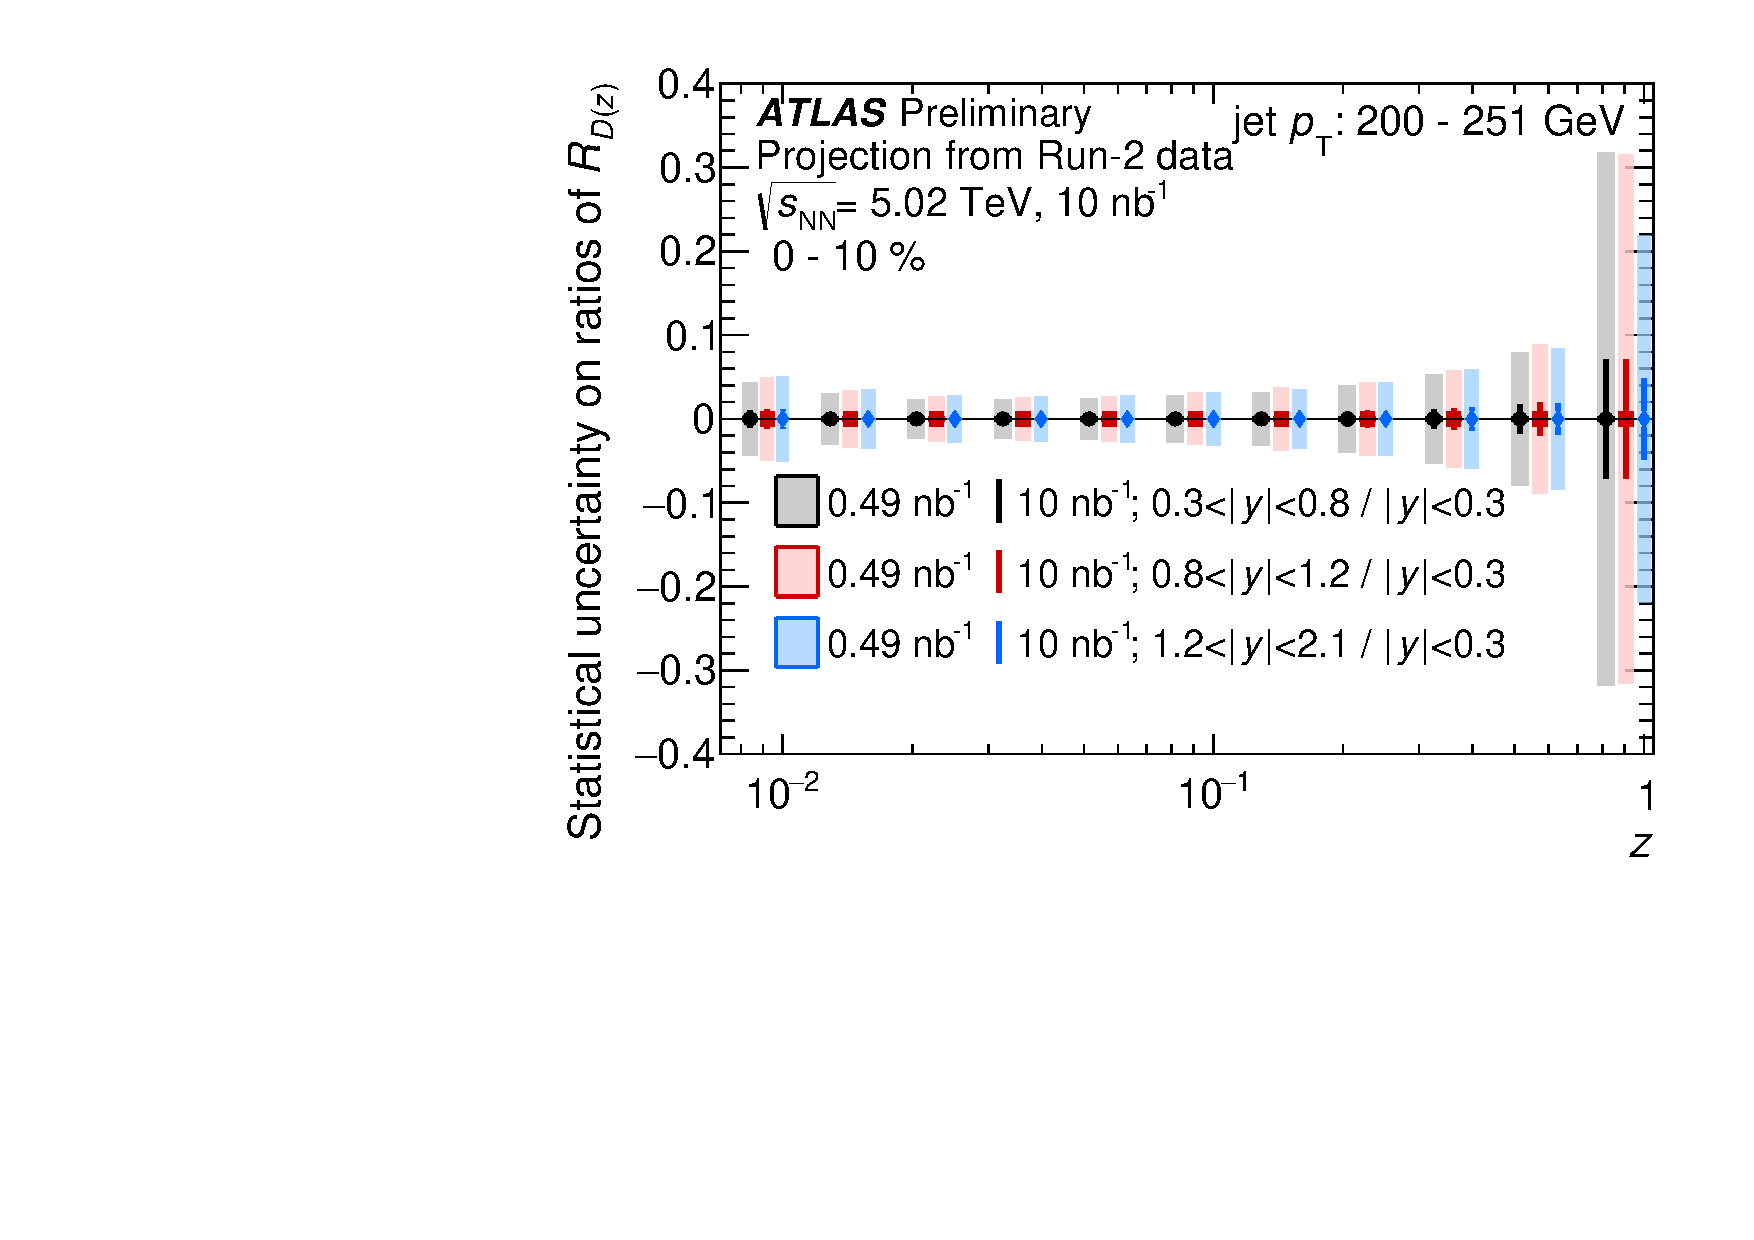
\includegraphics[width=.45\textwidth]{\main/jets/figures/atlas/fig_02b.pdf}
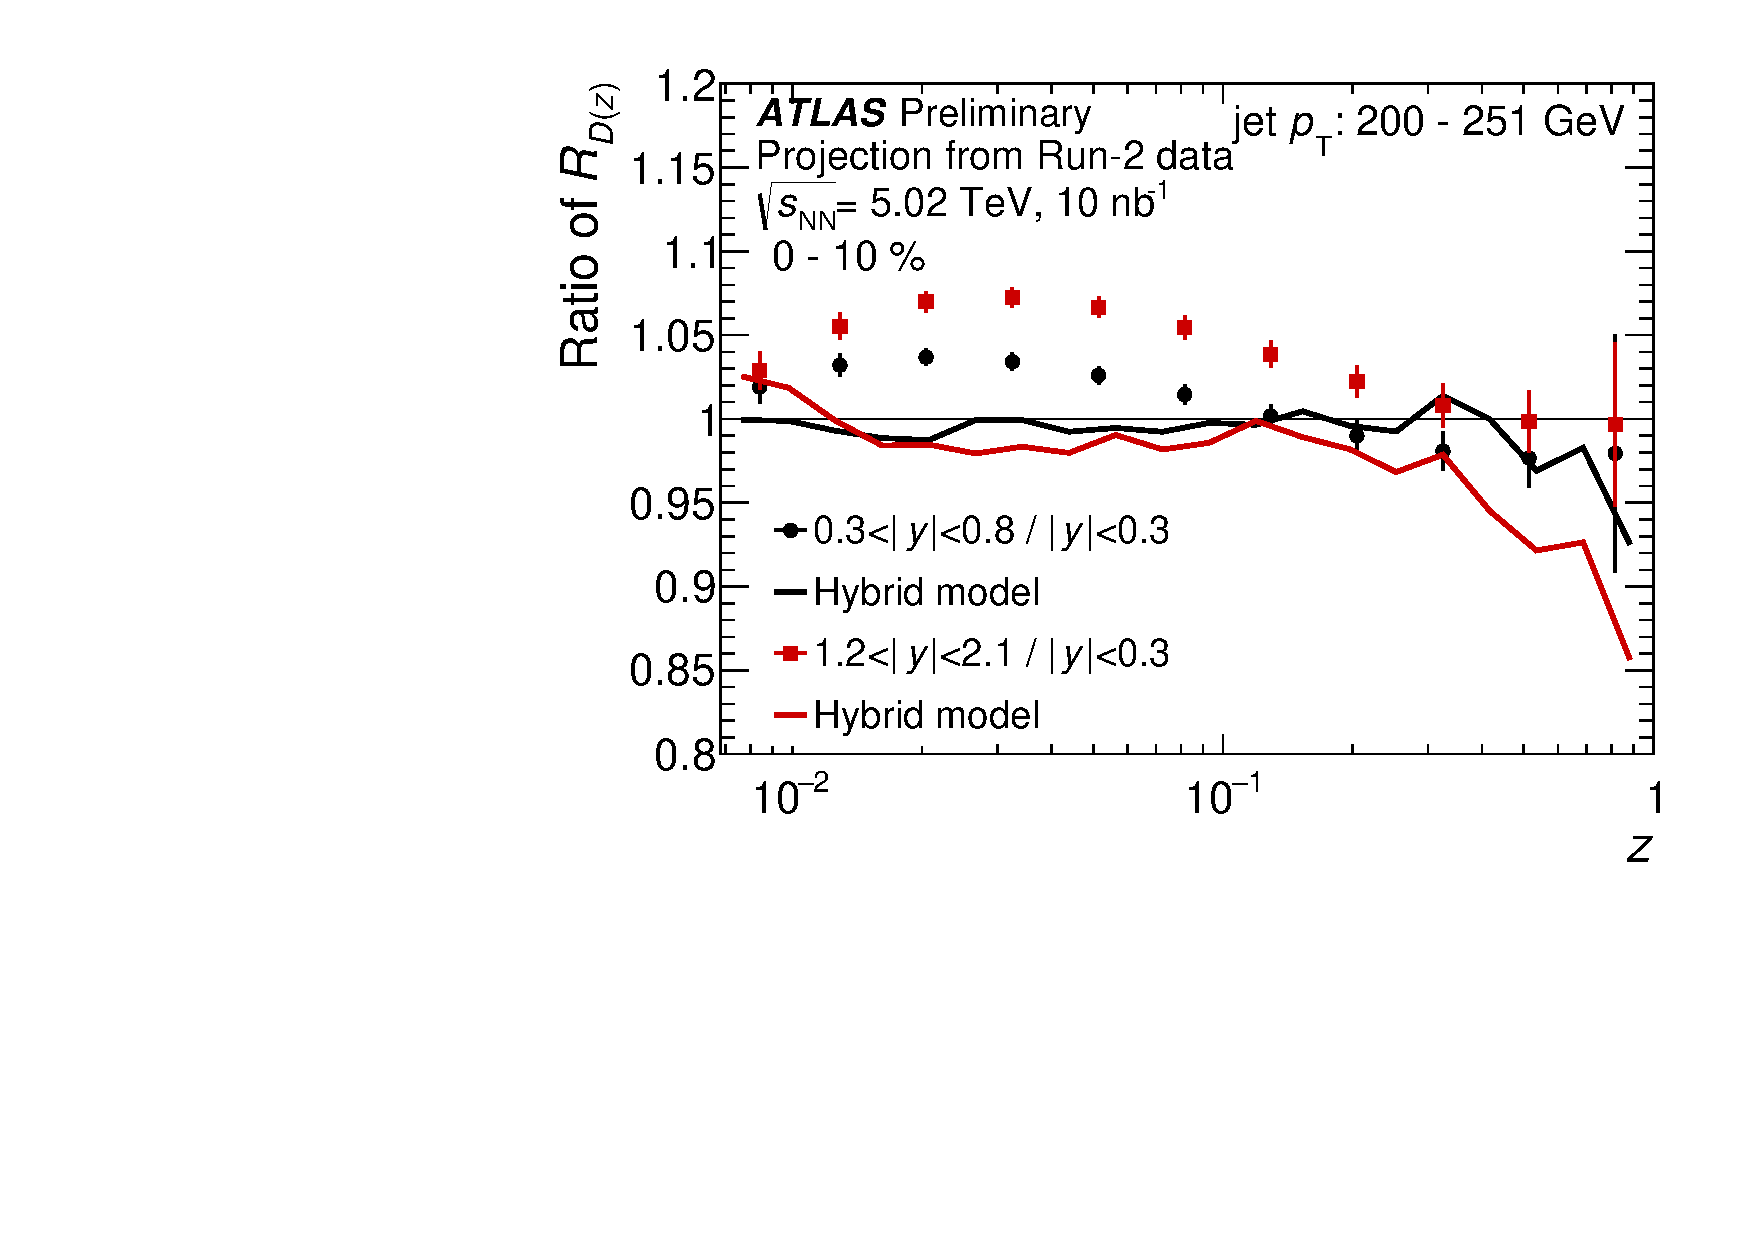
\includegraphics[width=.45\textwidth]{\main/jets/figures/atlas/fig_03b.pdf}
\caption{Projection of the precision that can be reached for the modification of jet fragmentation function, $R_{D(z)}$, measured in jet \pT\ interval $200-251$ \gevc. In the left panel the statistical uncertainty on the measurement with the shaded boxes corresponding to 0.49 $\mathrm{nb}^{-1}$ while the vertical bars are for 10 $\mathrm{nb}^{-1}$. The right panel shows a comparison of $R_{D(z)}$ with a theory model (see text for more details)~\cite{ATL-PHYS-PUB-2018-019}.}
\label{fig:jetDz}
\end{center}
\end{figure}

When interpreting the modification of inclusive jets one has to realize that by requiring a certain jet momentum range a different sample of partons initiating the jet is selected in pp and Pb--Pb collisions. Incorporation of this effect in model calculations introduces an additional uncertainty limiting the constraints that can be put on a model. This can be overcome by using the rare process of jets recoiling from photons. The expected performance of the radial \pT\ profile in jets recoiling from a high momentum photon at HL-LHC is shown in Fig.\ref{fig:jetshape}. The central values of the extrapolated spectra are obtained by smoothing the results from~\cite{Sirunyan:2018ncy} by a third order polynomial. The systematic uncertainties shown are obtained by reducing by a factor of two those from the 2015 Pb--Pb data results, considering the expected improvements on the jet energy scale and jet energy resolution uncertainties. The results show that the photon-tagged jet shape could be measured with high precision providing insights about the modification of the jet transverse structure of quark initiated jets in the strongly interacting medium.
%
\begin{figure}[!ht]
\begin{center}
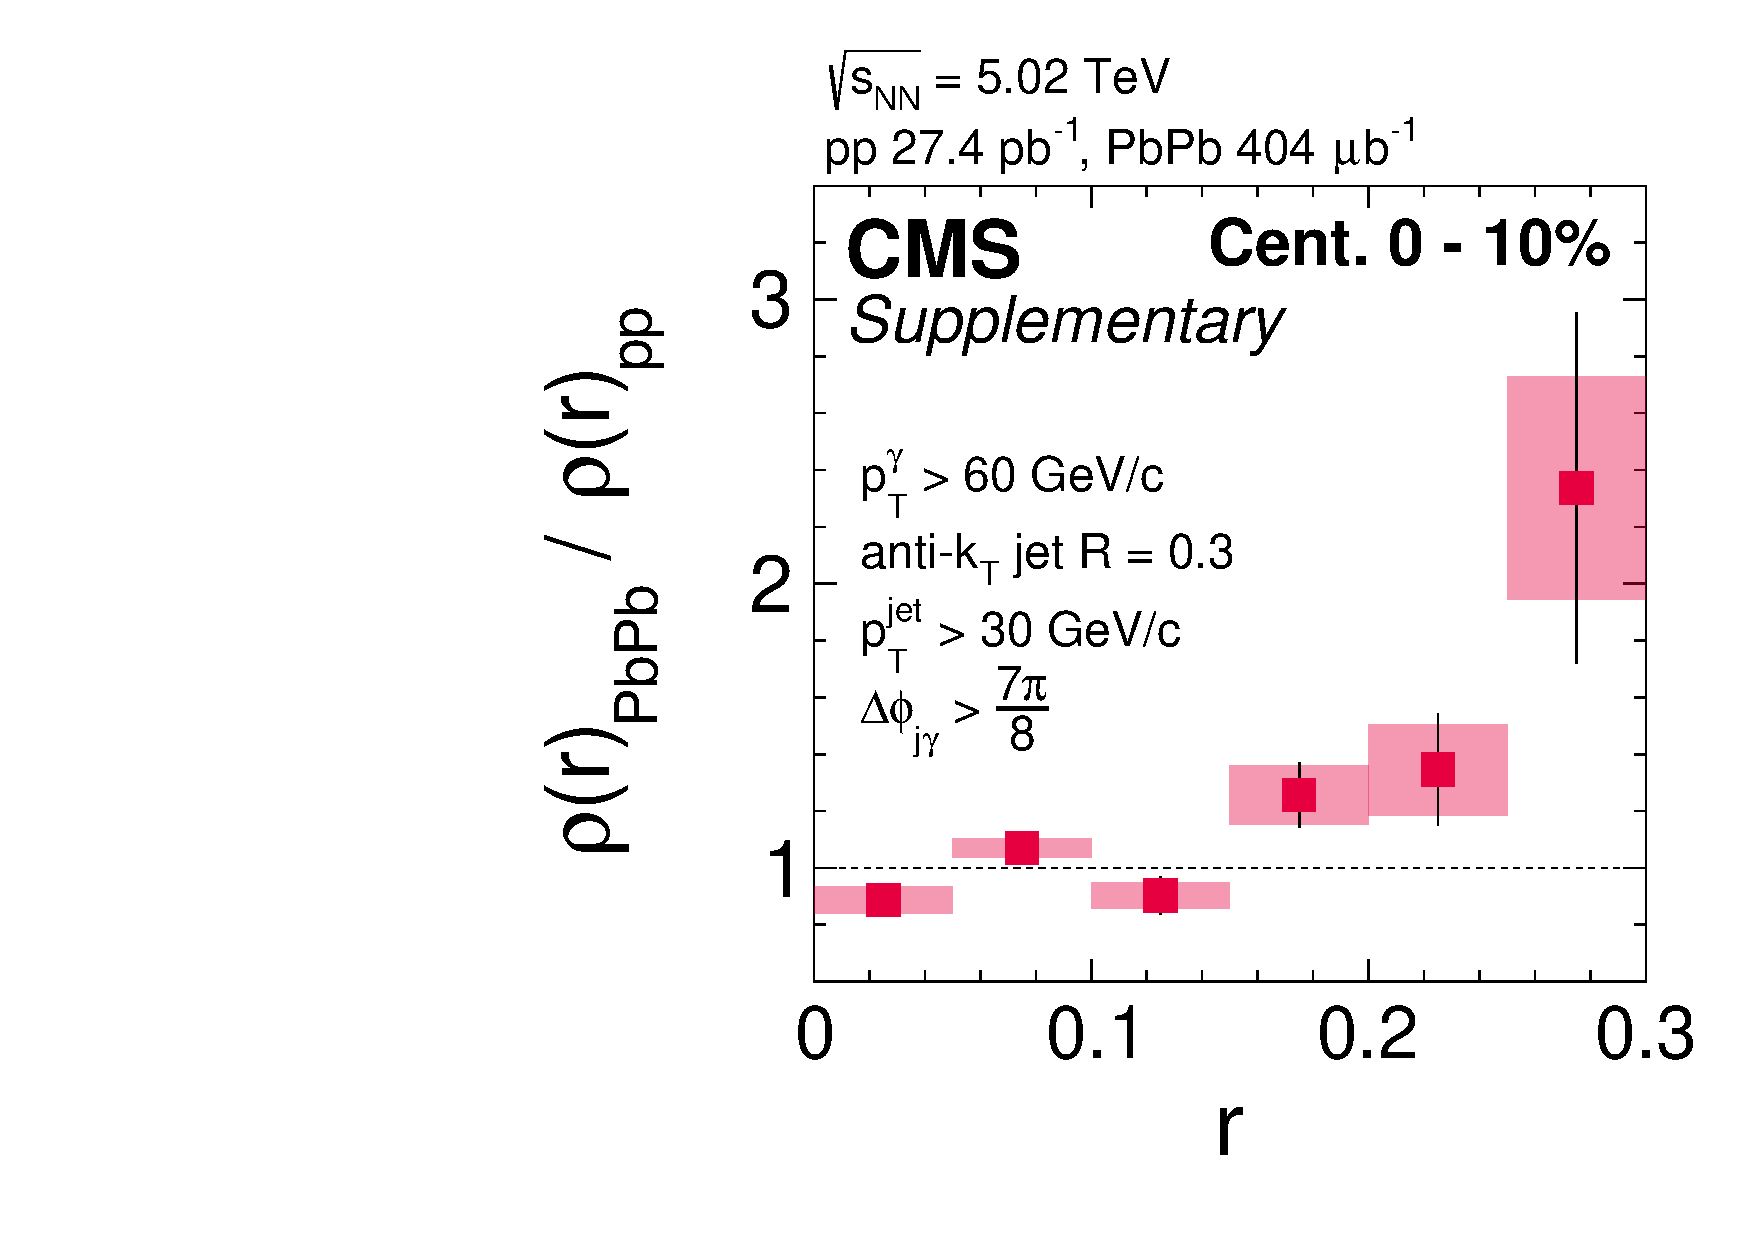
\includegraphics[width=.485\textwidth]{\main/jets/figures/cms/CMS-HIN-18-006_Figure-aux_004.pdf}
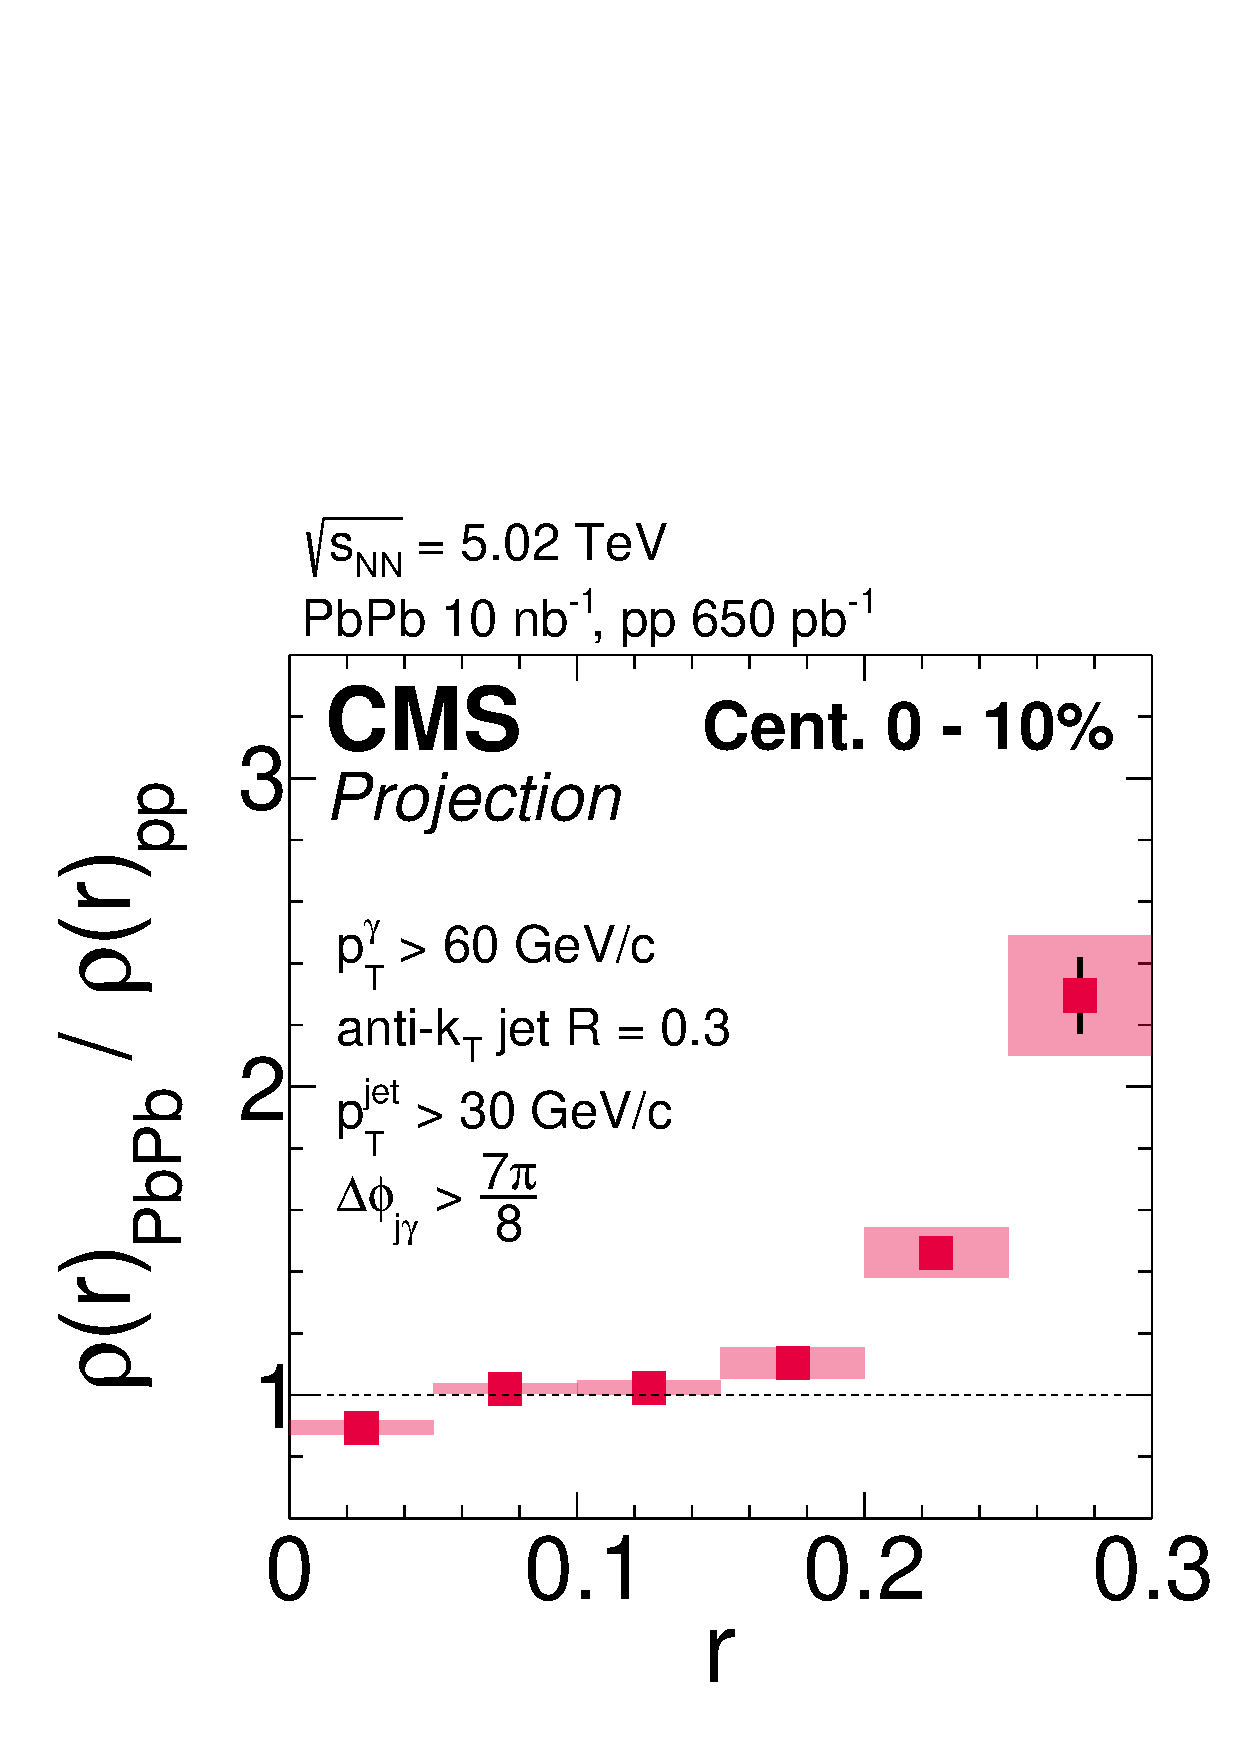
\includegraphics[width=.45\textwidth]{\main/jets/figures/cms/projection_js_ratioOnly_fit_pol3_sysReduced50Prct.pdf}
\caption{(Left Panel:) The ratio of measured photon-tagged jet shape in Pb--Pb and pp collisions with the 2015 Pb--Pb data~\cite{Sirunyan:2018ncy}. (Right Panel:) The expected performance of the jet shape ratio in the HL-LHC data, using a third-order polynomial for smoothing the data. [REF to be added when note is public]}
\label{fig:jetshape}
\end{center}
\end{figure}
%
Figure~\ref{fig:jetDzPh} shows the expected statistical precision of the fragmentation function on photon-tagged events. The larger data sample will allow enable the measurement for finer centrality selections with respect to the current preliminary results~\cite{ATLAS-CONF-2017-074} allowing to explore the temperature and path length dependence of jet quenching. 
\begin{figure}[!ht]
\begin{center}
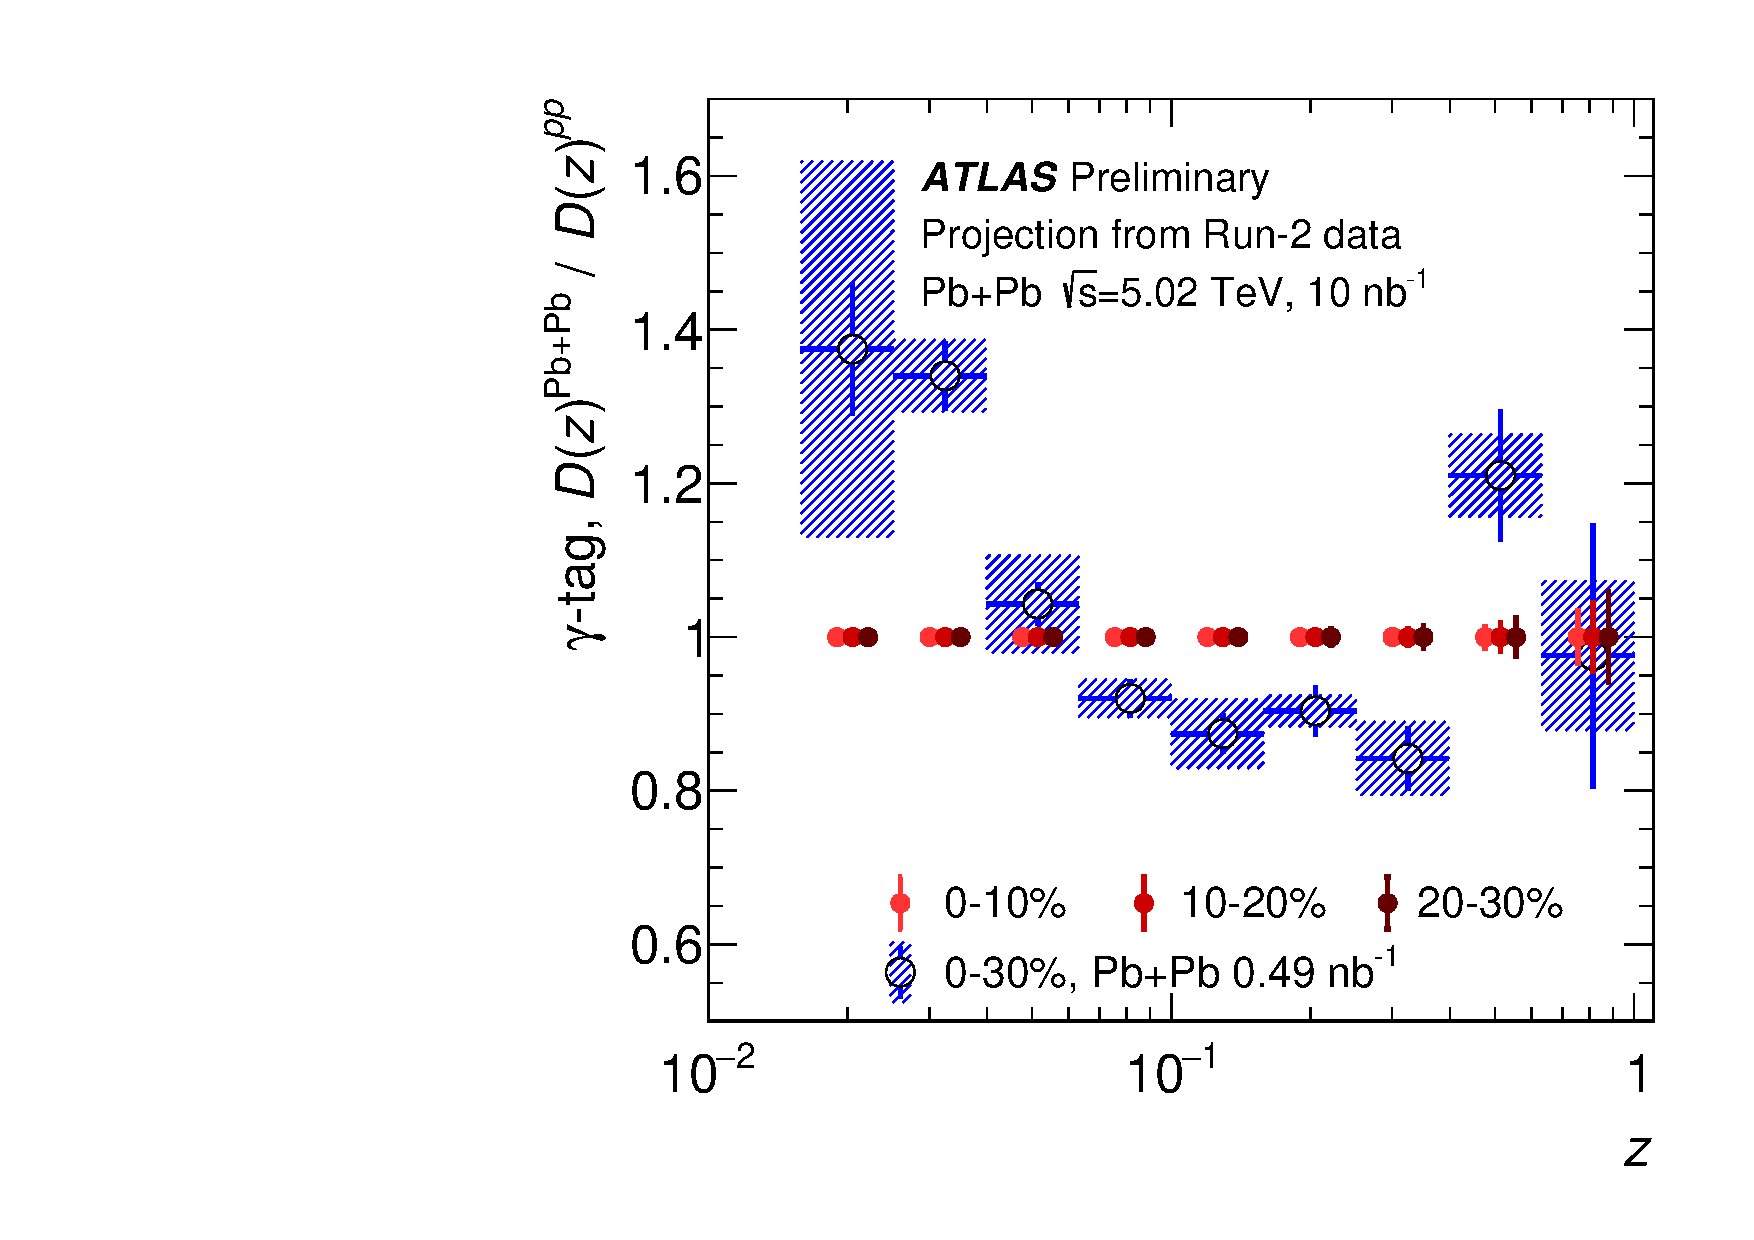
\includegraphics[width=.45\textwidth]{\main/jets/figures/atlas/fig_04a.pdf}
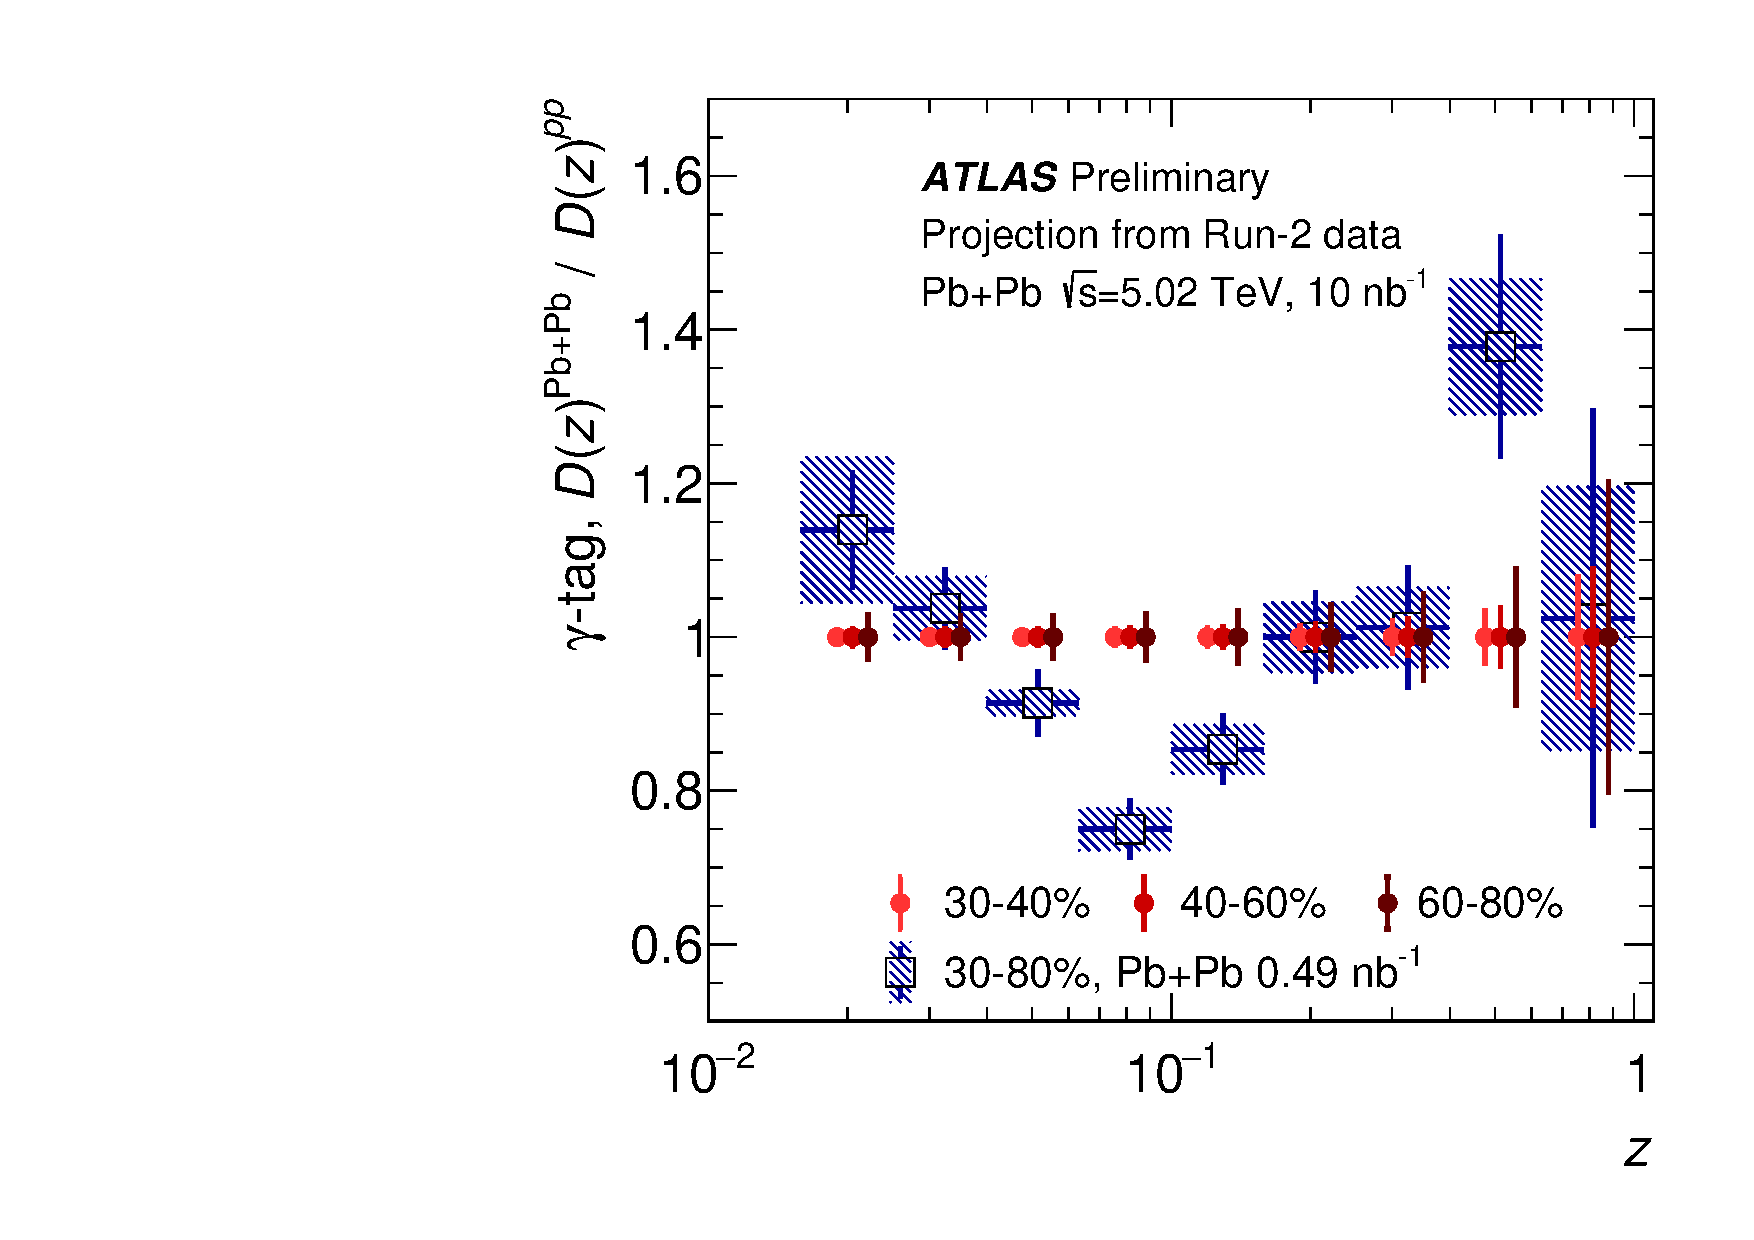
\includegraphics[width=.45\textwidth]{\main/jets/figures/atlas/fig_04b.pdf}
\caption{Projection of the statistical precision that can be reached for the ratio of jet fragmentation functions in Pb--Pb and pp collisions, $R_{D(z)}$, of jets recoiling from a photon. The left panel shows the projection for the most central collisions while the right panel for the more peripheral events~\cite{ATL-PHYS-PUB-2018-019}.}
\label{fig:jetDzPh}
\end{center}
\end{figure}


\subsubsection{Substructure with subjets}
Early hard splittings in a parton shower may result in two partons with high transverse momentum that are well separated in angle. 
Information about these leading partonic components can be obtained by removing the softer wide-angle radiation contributions. This is done through the use of a jet grooming algorithm called ``soft drop'', an extension of the modified mass drop tagger (mMDT), that attempt to split a single jet into two subjets, a process referred to as ``declustering''~\cite{Ellis:2009me,Butterworth:2008iy,Krohn:2009th,Dasgupta:2013ihk,Larkoski:2014wba}. For a parton shower in vacuum, these subjets provide access to the properties of the first splitting in the parton evolution~\cite{Altarelli:1977zs,Larkoski:2015lea}. Figure~\ref{fig:ZG} shows the expected performance for the momentum sharing fraction, $z_{\mathrm{g}}$~\cite{Larkoski:2015lea}, in the HL-LHC phase. The central values of $z_{\mathrm{g}}$ and jet mass are from previous CMS publications~\cite{Sirunyan:2017bsd,Sirunyan:2018gct}. The systematic uncertainties are reduced by a factor of two with respect to the results with 2015 Pb--Pb data due to the expected improvements on the jet energy scale and jet energy resolution uncertainties.  
While the current data is not precise enough to constrain the medium properties further, the expected luminosity at the HL-LHC will allow to do this in more detail as can be observed from the different results of the BDMPS~\cite{Mehtar-Tani:2016aco} and SCETg~\cite{Chien:2016led} calculations when the medium density ($\hat{q}$ for BDMPS and $g$ for SCETg) is varied. In addition, the expected precision will also allow to distinguish different physical mechanisms and scales relevant for jet quenching as is shown for the role of coherence in Fig.~\ref{fig:ZG} in the HT theoretical calculations~\cite{Chang:2017gkt}. A measurement of the groomed jet mass with the 2015 LHC Pb--Pb data already showed that jet quenching might cause an increase of high mass jets~\cite{Sirunyan:2018gct}. Figure~\ref{fig:Mass} shows the expected performance for the groomed jet mass at HL-LHC which will allow to measure the high mass region with higher precision.
\begin{figure}[!ht]
\begin{center}
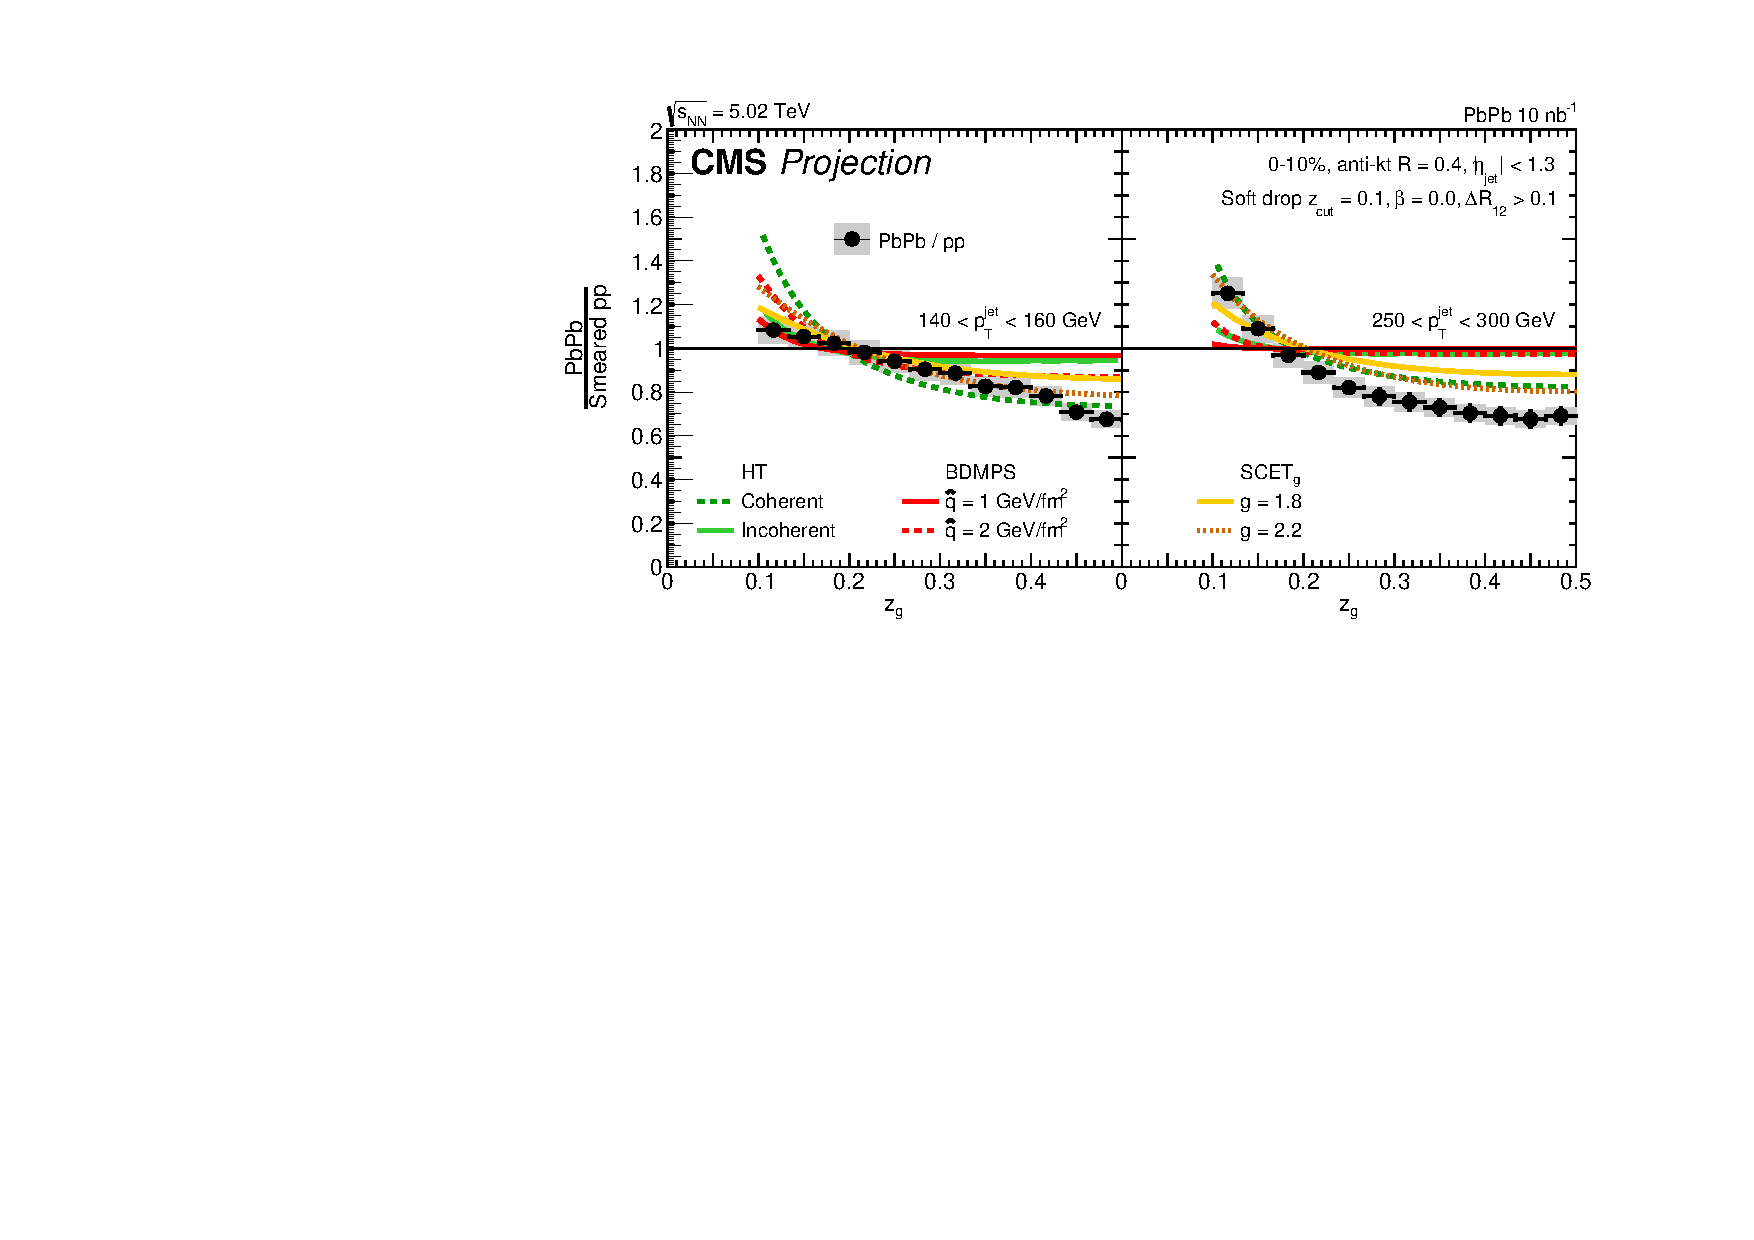
\includegraphics[width=.8\textwidth]{\main/jets/figures/cms/ZGMoneyPlot.pdf}
\caption{Performance of jet splitting function measurement with HL-LHC data in Pb--Pb collisions for two different selections in jet transverse momentum.~\cite{CMS-FTR-17-002:2017dec}}
\label{fig:ZG}
\end{center}
\end{figure}
%
\begin{figure}[!ht]
\begin{center}
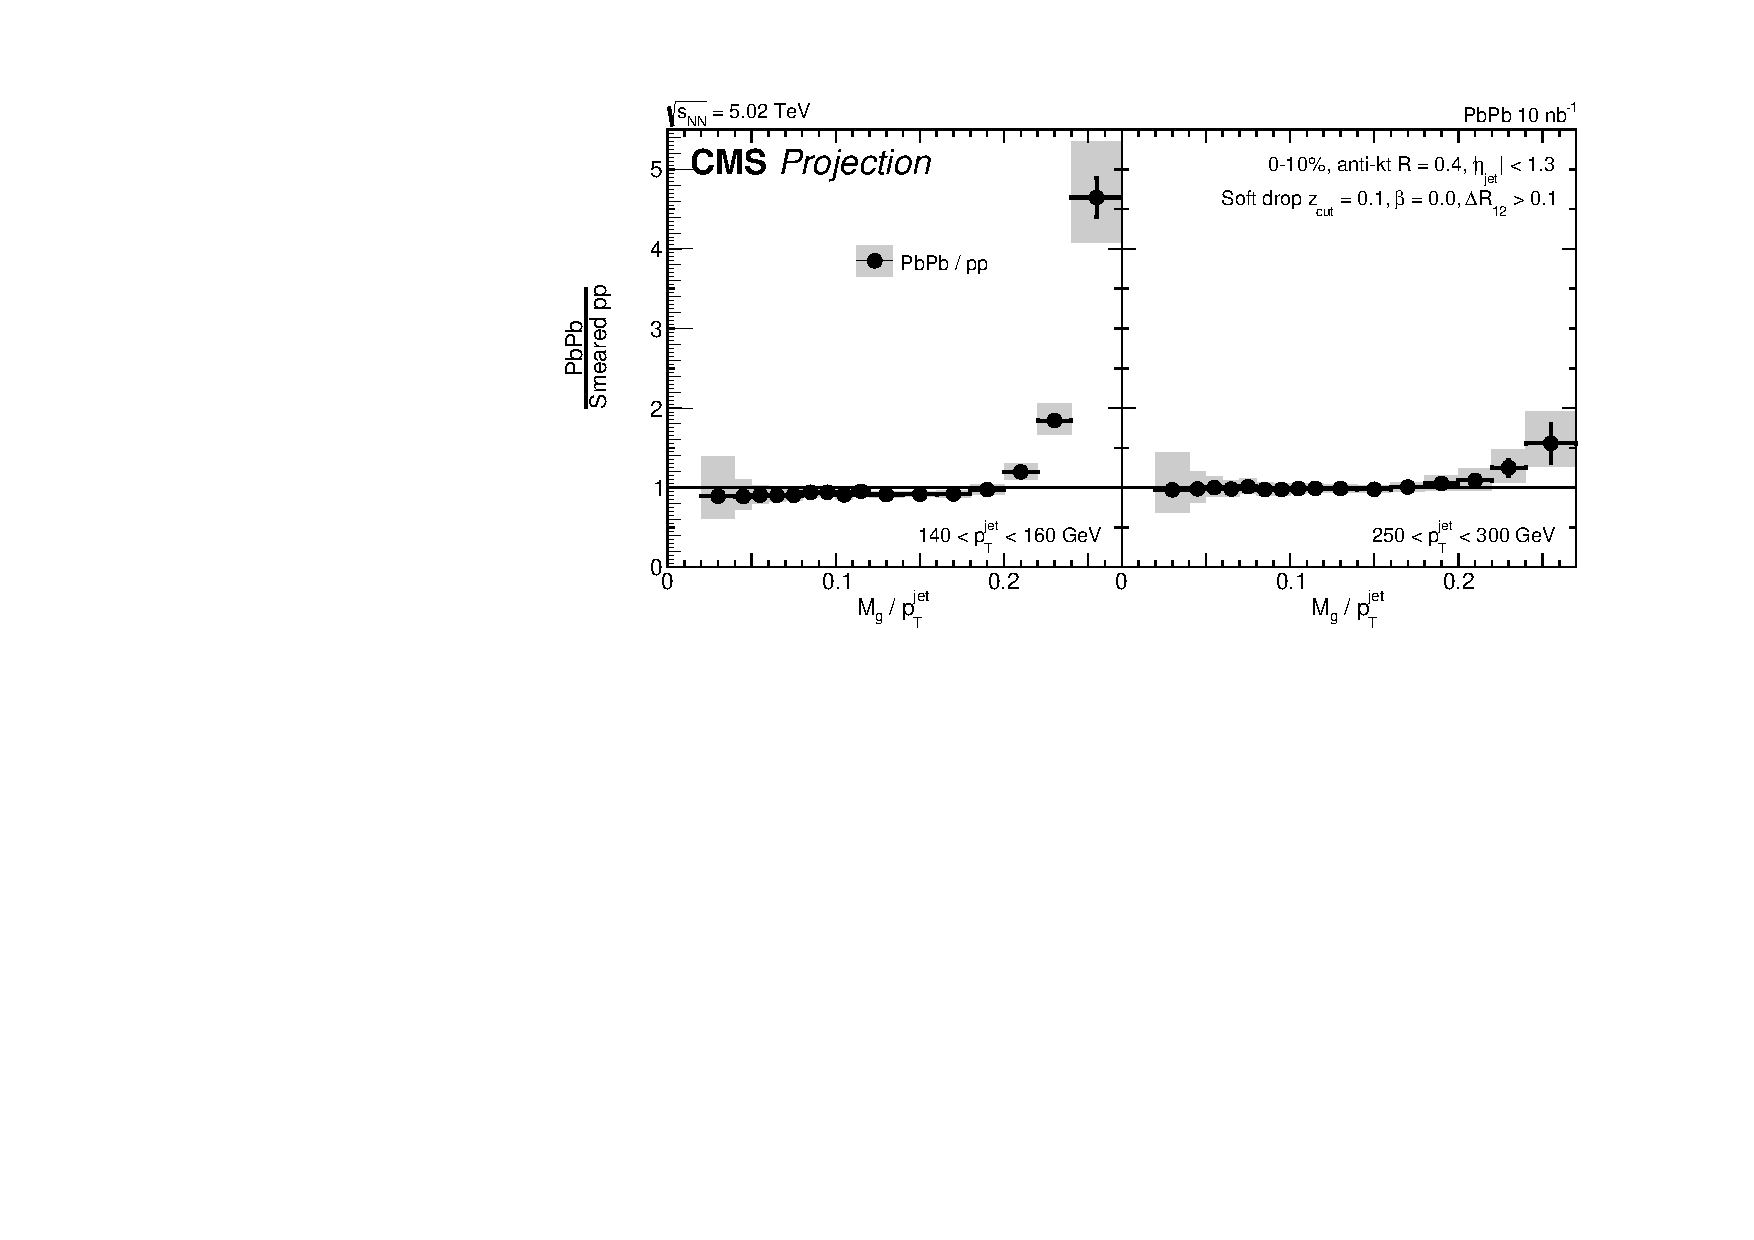
\includegraphics[width=.8\textwidth]{\main/jets/figures/cms/MGMoneyPlot_0.pdf}
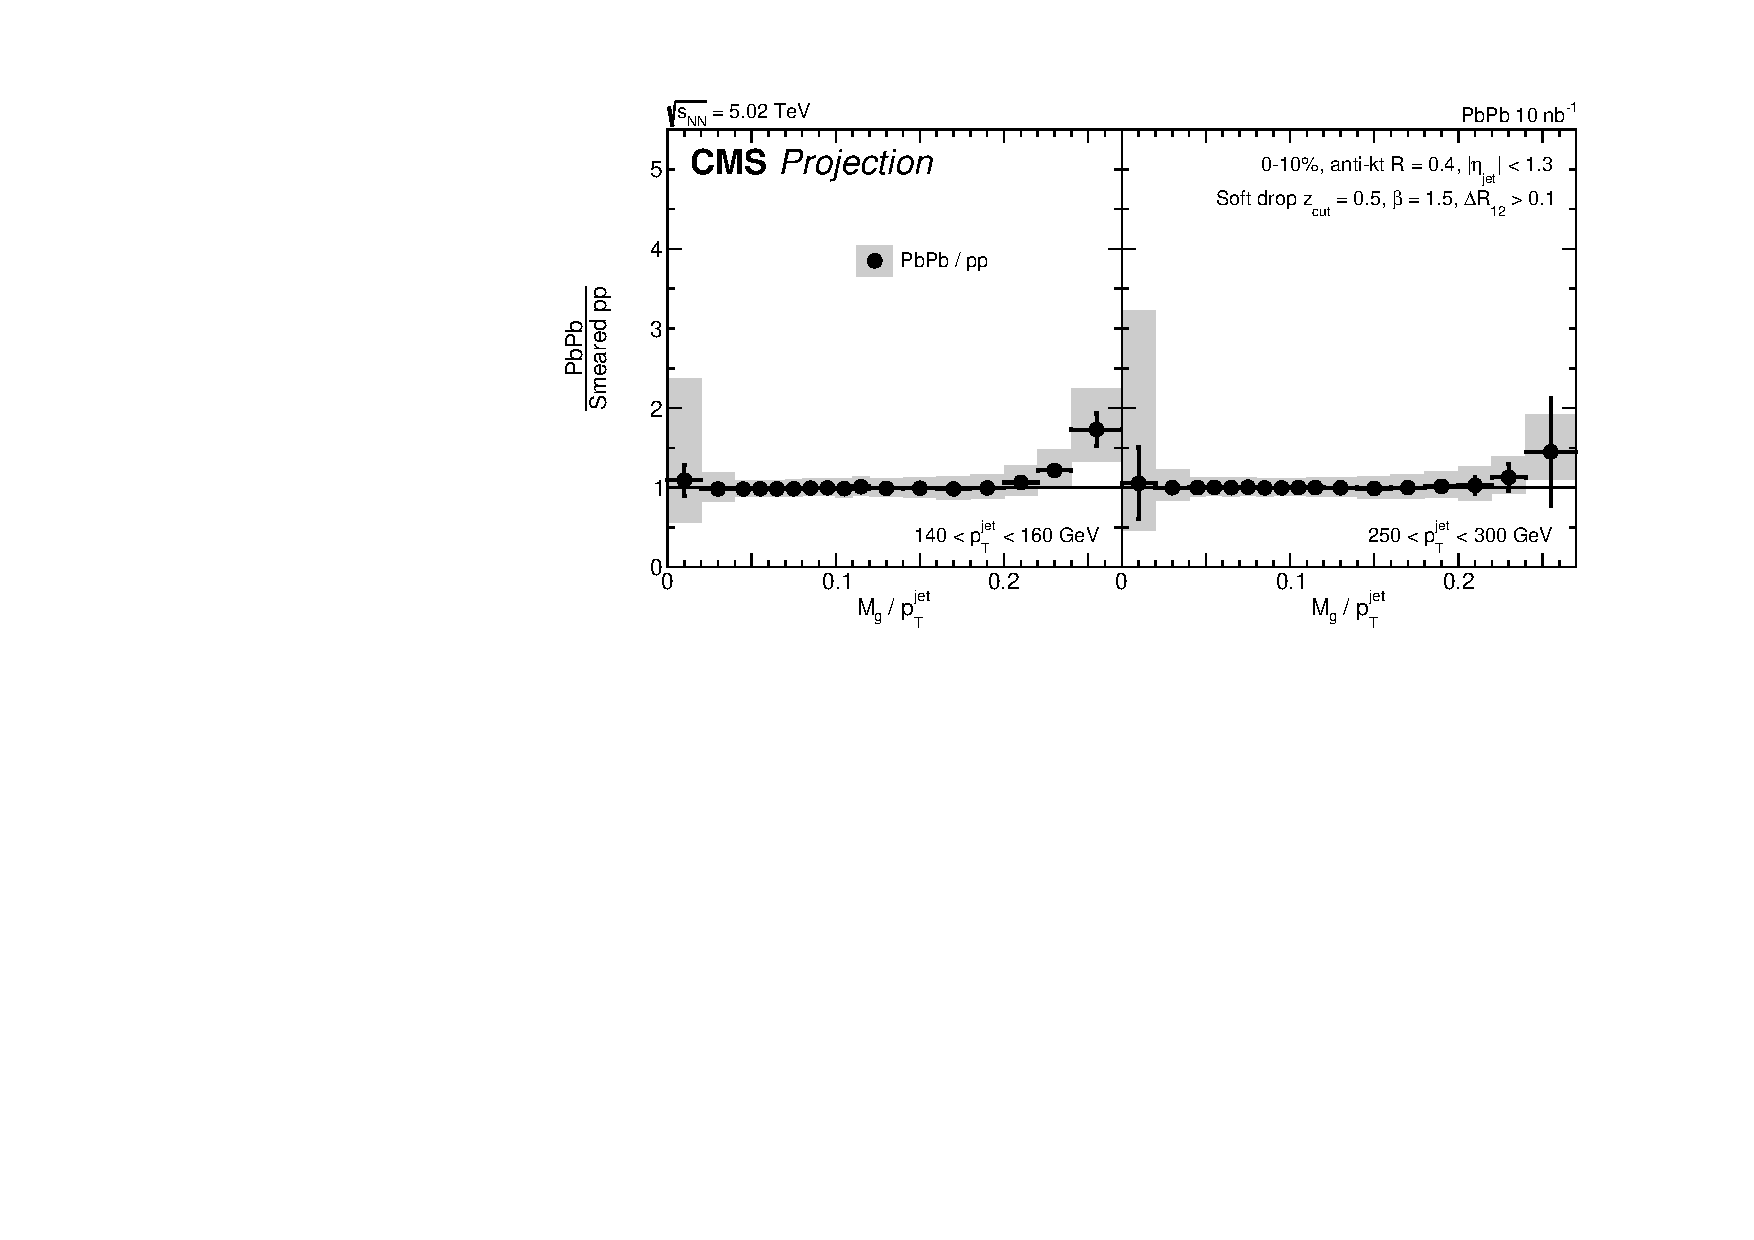
\includegraphics[width=.8\textwidth]{\main/jets/figures/cms/MGMoneyPlot_7.pdf}
\caption{Jet mass distribution with grooming setting $(z_{cut},\beta)=(0.1,0.0)$ (Upper panels) and $(z_{cut},\beta)=(0.5,1.5)$ (Lower panels).~\cite{CMS-FTR-17-002:2017dec}}
\label{fig:Mass}
\end{center}
\end{figure}


%\clearpage
\newpage
\subsubsection{Radiation phase space with Lund diagram}

Recently, a theoretical representation of the radiation phase space within jets inspired by Lund diagrams~\cite{Andersson:1988gp} has been proposed~\cite{Andrews:2018jcm} to study medium modification of the radiation pattern. The so-called Lund jet plane~\cite{Dreyer:2018nbf} - a portrayal of the internal structure of jets - was designed to build a conceptual connection between manually constructed observables and approaches that use Machine Learning techniques to study QCD jets and/or discriminate between signal and background jets.
The diagram is constructed by mapping the available phase-space within a jet to a triangle in a two dimensional (logarithmic) plane that shows the transverse momentum and the angle of any given emission with respect to its emitter.
Such a triangular diagram, a representation of the radiation within any given jet, can be created through repeated Cambridge/Aachen declustering.

To demonstrate the potential of future measurements at the LHC we constructed Lund diagrams using the \jewel\ Monte Carlo event generator~\cite{Zapp:2013vla}.
To study the differences in the Lund diagram due to medium effects the results are compared to a vacuum reference (jets produced in \pp\ collisions). For the simulations the \jewel
 generator with the default settings is used without the optional calculation of the so-called medium response retaining the partons / scattering centres that interacted with the jet was not used (i.e. {\it recoils off} setting of the MC generator was used).
%Jets were reconstructed with the \akt\ algorithm~\cite{Cacciari:2008gp} with resolution parameter $R=0.4$ using \fastjet\ package~\cite{Cacciari:2011ma,Cacciari:2005hq}.
%Jets retained for the substructure analysis were required to have their centroid within two units of pseudorapidity around $\eta_{\rm lab}=0$ (i.e. $|\eta^{\rm jet}| < 2$).
The substructure of jets was analysed by reclustering the constituents of the jet with the Cambridge/Aachen (C/A) algorithm as implemented in the \fastjet\ package~\cite{Cacciari:2011ma,Cacciari:2005hq} for two selections of jet \pt\ 80--120~$\gevc$ and 200--250~$\gevc$.

\begin{figure}[ht]
	\centering
	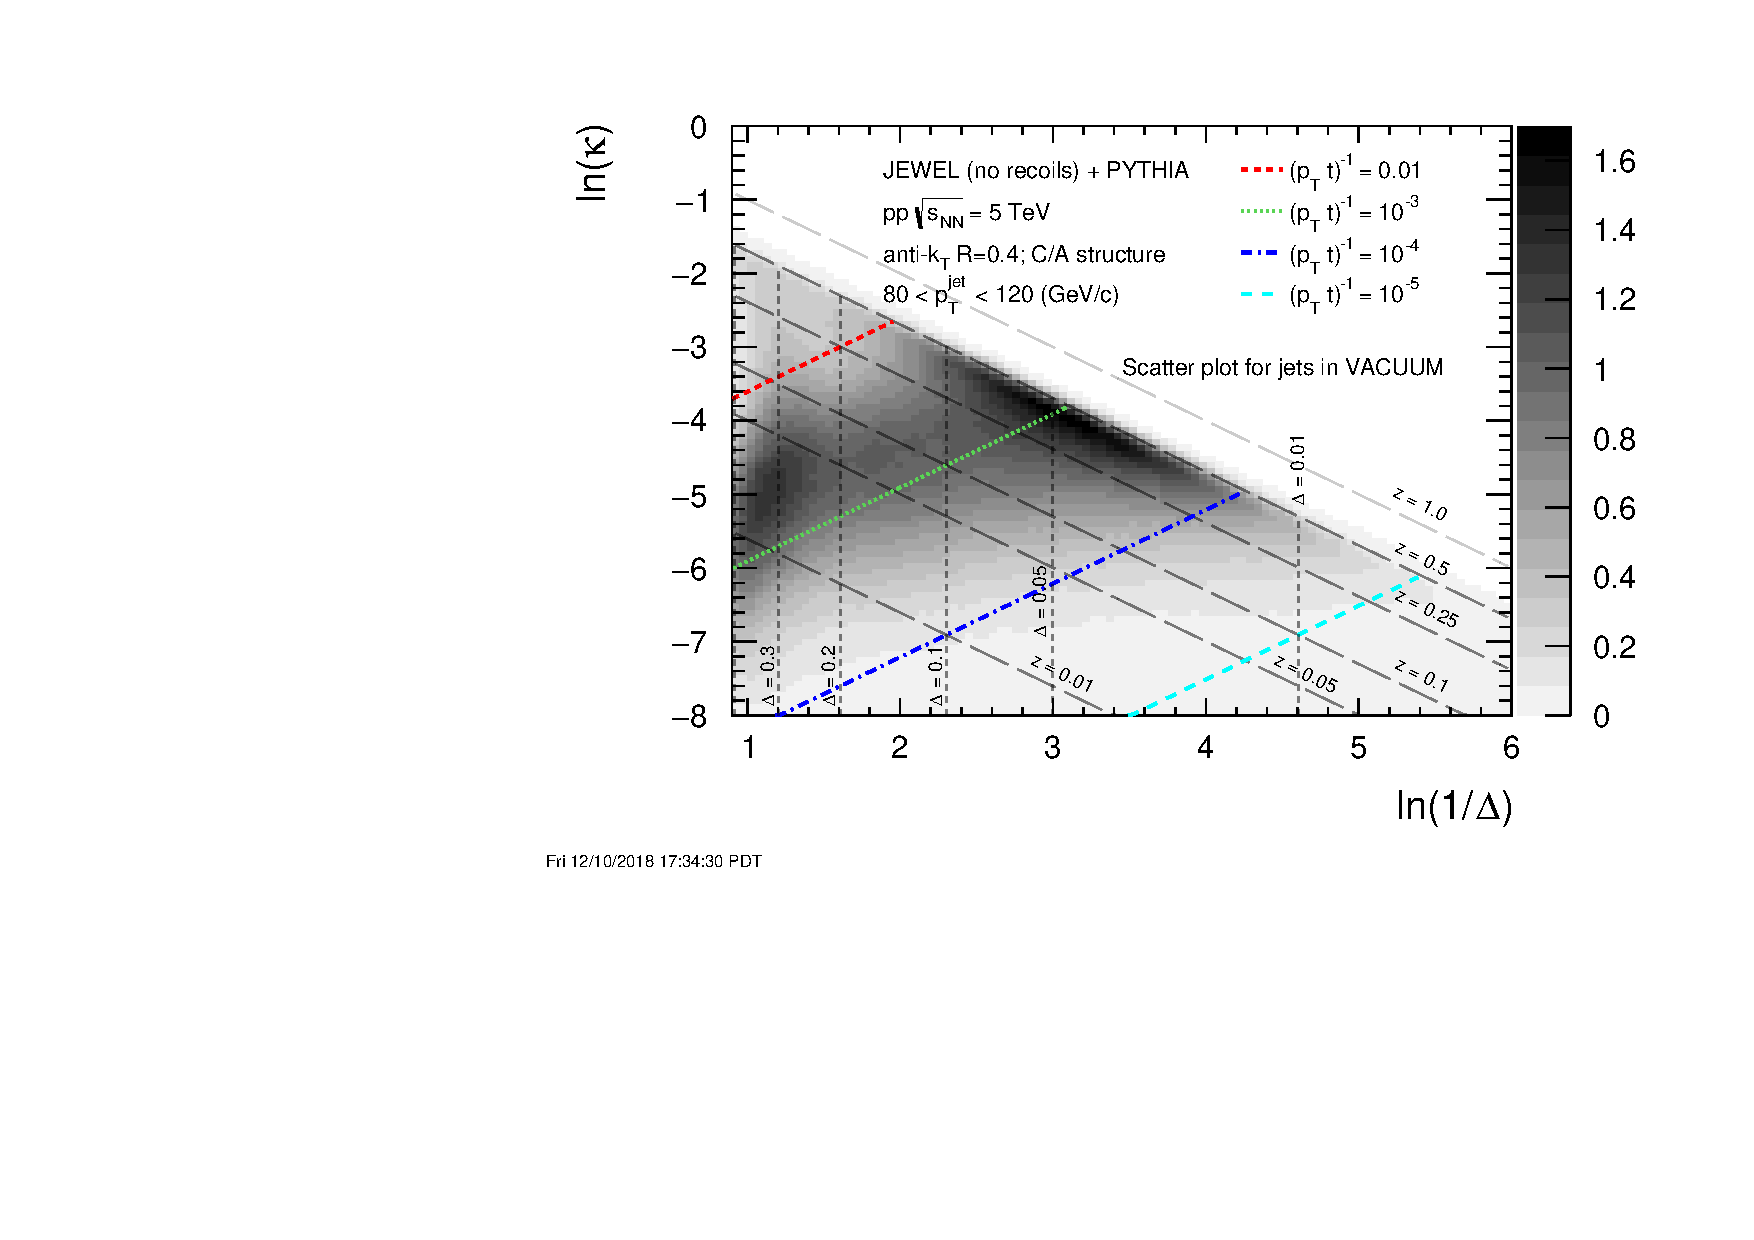
\includegraphics[width=0.45\textwidth,page=1]{\main/jets/figures/lund/lund_t}
	\includegraphics[width=0.45\textwidth,page=2]{\main/jets/figures/lund/lund_t}
	\includegraphics[width=0.45\textwidth,page=4]{\main/jets/figures/lund/lund_t}
	\includegraphics[width=0.45\textwidth,page=5]{\main/jets/figures/lund/lund_t}
	\caption{The density of points of a Lund diagram for anti-\kT\ $R=0.4$ jets for two \pt\ selections: $80 < \pt\ < 120$ \gevc\ in the upper row and $200 < \pt\ < 250$ \gevc\ in the lower row. Result of the \jewel\ Monte Carlo generator with left column: jets in \pp\ collisions; Right column: jets from Pb--Pb collisions - some with in-medium modifications. Each of the density plots shows curves of the average quantities of the densities over the other axis.}
	\label{fig:Lund_jets}
\end{figure}

The Lund diagram density can be constructed experimentally and compared to analytic predictions and parton-shower Monte-Carlo simulations, such as \jewel. For this purpose a density map of points (emissions) is defined following formulations in~\cite{Dreyer:2018nbf}: 
\begin{equation}
\bar{\rho}(\Delta, \kappa) = \frac{1}{N_{\rm jet}} \frac{\mathrm{d}n_{\rm emission}}{\mathrm{d} \ln \kappa~\mathrm{d} \ln 1/\Delta},
\end{equation}
where for two clusters $1$ and $2$ labelled such that $p_{\rm T,1} > p_{\rm T,2}$, $\Delta^{2} = (y_1 - y_2)^2 + (\varphi_1 - \varphi_2)^2$ with $\varphi$ being the azimuthal angle and $y$ the rapidity of a cluster, and $\kappa=\frac{p_{\rm T,2}}{p_{\rm T,1} + p_{\rm T,2}}\Delta$. Figure~\ref{fig:Lund_jets} shows the density $\bar{\rho}$ from the \jewel\ simulation without (left panels) and with (right panels) medium effects. 
The $z_{\rm g}$ variable which was defined in~\cite{Larkoski:2015lea} and studied in heavy-ion collisions~\cite{Sirunyan:2017bsd} is related to the variables in the Lund plane in the following way: $z_{\mathrm{g}} = \kappa/\Delta$ resulting in diagonal lines with negative slope in the Lund diagram for a constant value of $z_\mathrm{g}$.
%
\begin{figure}[htbp]
	\centering
	\includegraphics[width=0.45\textwidth,page=3]{\main/jets/figures/lund/lund_t}
	\includegraphics[width=0.45\textwidth,page=6]{\main/jets/figures/lund/lund_t}
	\caption{Result of the JEWEL+PYTHIA MC simulation: MEDIUM-VACUUM difference of the calculations shown in Fig.~\ref{fig:Lund_jets} for two jet \pt\ selections.}
	\label{fig:Lund_jets_vac_med}
\end{figure}

The effect of jet quenching on the Lund diagram is quantified by taking the difference between the diagram with and without medium effects as shown in Fig.~\ref{fig:Lund_jets_vac_med} for the two transverse momentum ranges considered in this study. 
The average density integrated over $\ln \kappa$ calculated for Pb--Pb (MEDIUM) case shows little deviation from the pp (VACUUM) reference. 
The most pronounced differences between VACUUM and MEDIUM calculations are visible for the region of $-3 < \ln \kappa < -3$ and large $\ln 1\Delta$ which correspond to the hard-collinear splittings (Region-A), and a band along $\ln 1/\Delta$ for small $\ln \kappa$ (Region-B): $-5 < \ln \kappa < -6$ for the lower \pt\ selection and $-5.5 < \ln \kappa < -7$ for higher \pt\ jets; that corresponds to an enhancement of soft (moderate $\ln 1/\Delta$) and hard collinear splittings (large $\ln 1/\Delta$). 
%Whereas the average density along $\ln 1/\Delta$ for the MEDIUM case shows significant deviations from VACUUM for $\ln 1/\Delta < 3$ (Region-A) for jets in the lower \pt\ range and for $\ln 1/\Delta < 4$ (Region-B) for higher \pt\ jets. 
These observations are consistent with soft and hard collinear splittings being modified by the medium.

To illustrate the different modifications of the Lund diagram density for the two regions identified in Fig.~\ref{fig:Lund_jets_vac_med}, projections along $\ln 1/\Delta$ are shown in Fig.~\ref{fig:Lund_projections}. For Region-A we observe 30\%-40\% depletion of splittings for the MEDIUM case whereas in Region-B a moderate increase of splittings induced by the medium is visible. The depletion in Region-A is consistent a sample of more collimated jets consistent with previous measurements in heavy-ion collisions~\cite{Acharya:2018uvf,Sirunyan:2018jqr}. The increase seen in Region-B is consistent with a small in-medium enhancement of splittings with moderate dependency on the angle of the splitting but favoring the soft collinear medium-induced radiation (moderate $ln 1/\Delta$).
\begin{figure}[htbp]
	\centering
	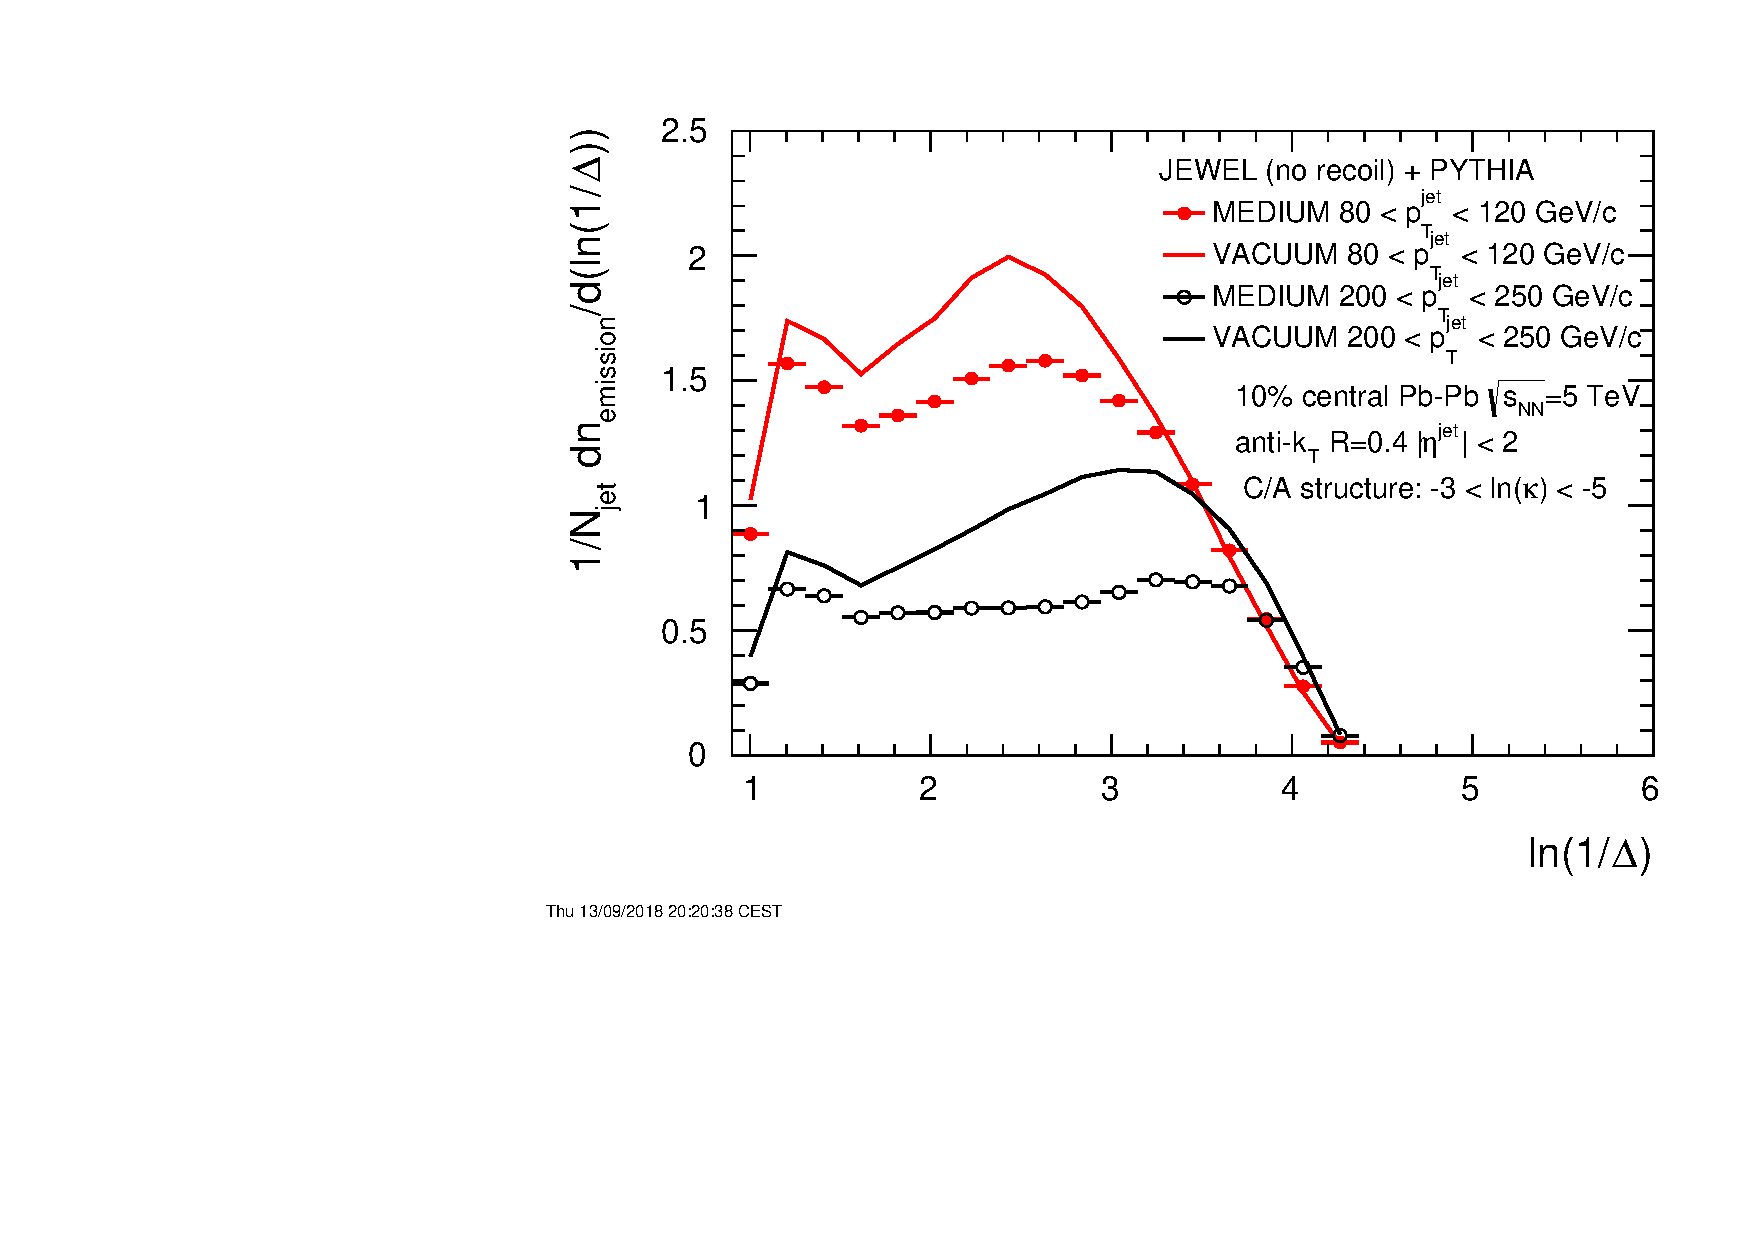
\includegraphics[width=0.49\textwidth,page=1]{\main/jets/figures/lund/lund_projections}
	\includegraphics[width=0.49\textwidth,page=2]{\main/jets/figures/lund/lund_projections}
	\caption{Projections of the lund diagram along the angular separation $\ln 1/\Delta$ of the splittings for the two selections of jet \pt. In-medium suppression of splittings for moderate $\ln{\kappa}$ according to \jewel\ (left). Enhancement for small $\ln{\kappa}$ (right).}
	\label{fig:Lund_projections}
\end{figure}

%\paragraph{Modifications of splittings and formation time}

%{\it MP: text is a placeholder here...}
As discussed in Ref.~\cite{Andrews:2018jcm} specific regions in the Lund plane are sensitive to different type of parton splittings. 
These regions can be identified by selecting the desired area using linear functions $\ln\kappa = \ln1/\Delta + \ln \frac{1}{p_{\rm T} t}$, where $t$ is related to the decoherence time (thus formation time).
Depending on the selection, different formation times are probed and splittings will occur within or outside the medium.
We investigate three regions of the Lund plane according to a selection of diagonal lines for different $\frac{1}{p_{\rm T} t}$ indicated in Fig.~\ref{fig:Lund_jets}.
The density of the splittings is projected along the momentum imbalance $z = p_{\rm T,2}/(p_{\rm T,1} + p_{\rm T,2})$.
In Fig.~\ref{fig:Lund_projections_z} we show the relative difference of the splitting density $\Delta_{\rm}\bar{\rho} = (\bar{\rho}_{\mathrm med} - \bar{\rho}_{\mathrm vac})/\bar{\rho}_{\mathrm vac}$.
For small formation times the splitting density is suppressed for the in-medium calculations whereas for large $p_{\rm T} t$ the modification is smaller and even slightly enhanced for large formation times.
This is consistent with the expectation that for large formation times the medium effects should be of smaller magnitude as compared to splittings formed early.
%
\begin{figure}[ht]
	\centering
	\includegraphics[width=0.32\textwidth,page=4]{\main/jets/figures/lund/lund_t_z}
	\includegraphics[width=0.32\textwidth,page=8]{\main/jets/figures/lund/lund_t_z}
	\includegraphics[width=0.32\textwidth,page=9]{\main/jets/figures/lund/lund_t_z}
	\caption{Projections of the relative difference of the Lund diagram onto momentum imbalance of the splittings for two selections of jet \pt\ and selections of $\frac{1}{p_{\rm T} t}$.
	Left: relative difference for low-\pt\ jets for three selections of $\frac{1}{p_{\rm T} t}$.
	Middle: relative difference for high-\pt\ jets for three selections of $\frac{1}{p_{\rm T} t}$.
 Right: comparison of low- and high-\pt\ for two selections of $\frac{1}{p_{\rm T} t}$.
	}
	\label{fig:Lund_projections_z}
\end{figure}

%\paragraph{Projection along angular separation}
%The most pronounced differences between VACUUM and MEDIUM calculations shown in Fig.~\ref{fig:Lund_jets_vac_med} are visible for the region of $-3 < \ln \kappa < -3$ and large $\ln 1\Delta$ which correspond to the hard-collinear splittings (Region-A), and a band along $\ln 1/\Delta$ for small $\ln \kappa$ (Region-B): $-5 < \ln \kappa < -6$ for the lower \pt\ selection and $-5.5 < \ln \kappa < -7$ for higher \pt\ jets; that corresponds to an enhancement of soft (moderate $\ln 1/\Delta$) and hard collinear splittings (large $\ln 1/\Delta$).




